\section{Página de edición de una ley de lex.gal}
\label{PEdicionLexGal}

\begin{figure}[H]
\centerline{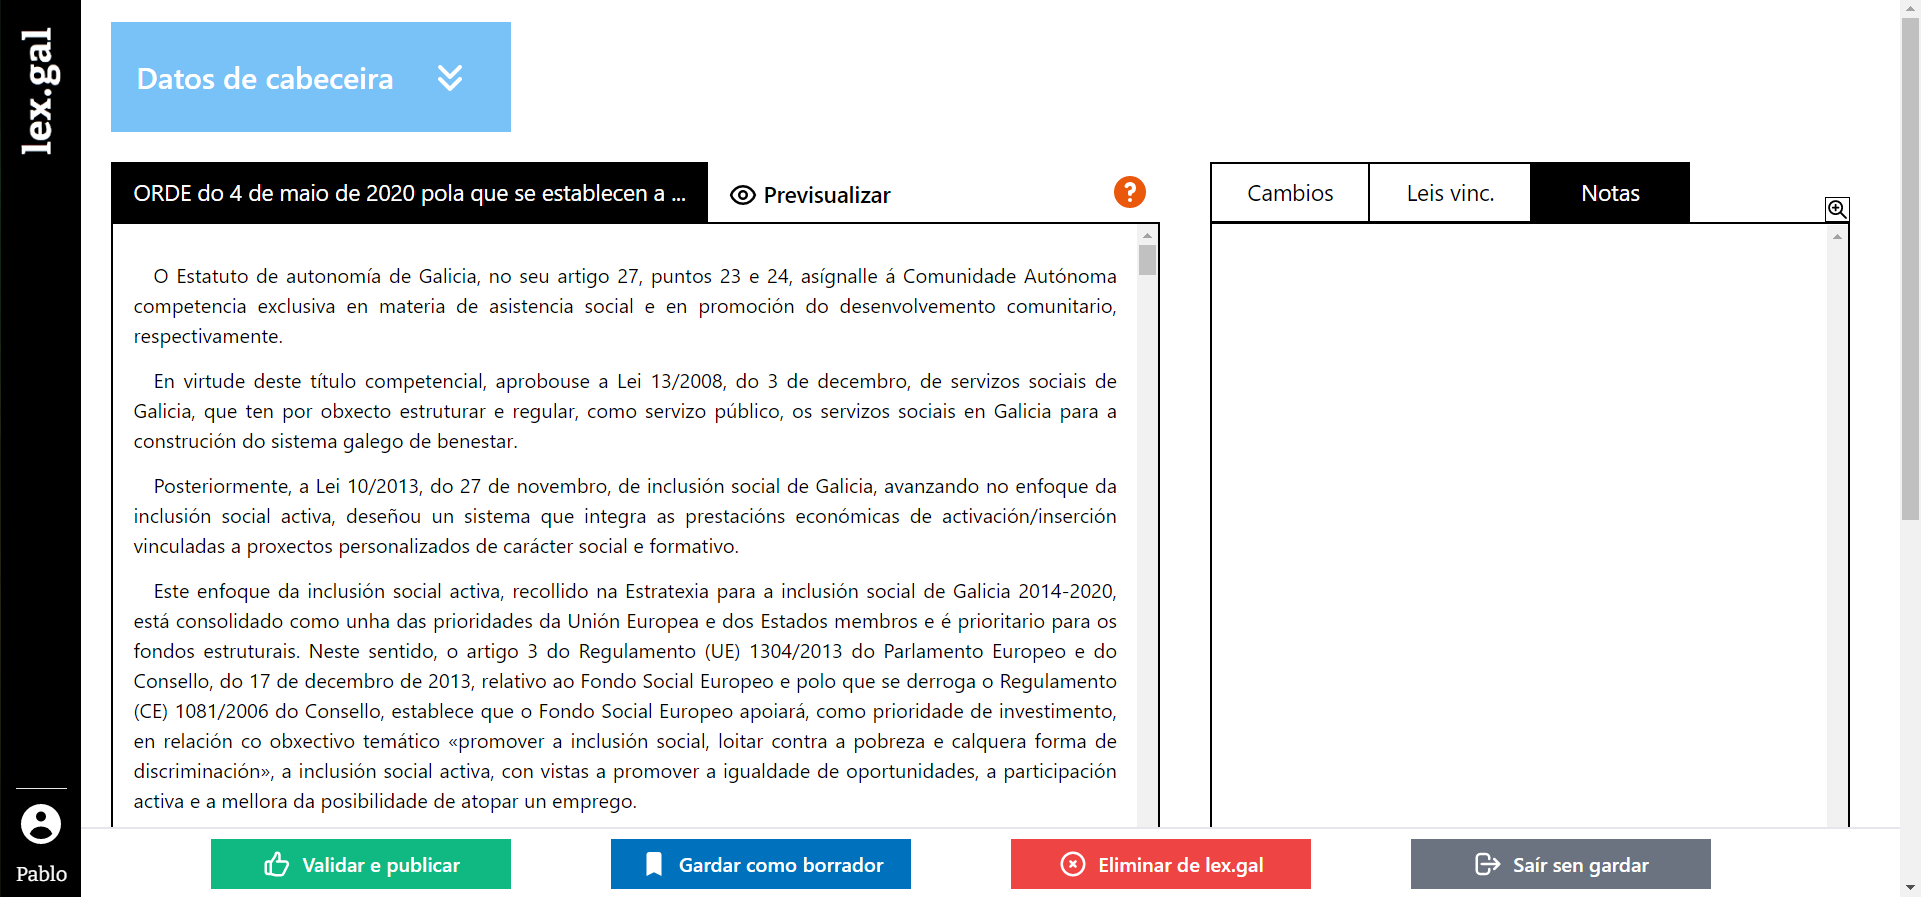
\includegraphics[width=15cm]{figuras/manualUsuario/EditarPrincipal.PNG}}
\caption{Página de edición de una ley de lex.gal.}
\label{enlaceEdicionLexGal}
\end{figure}

La página de edición, que se puede ver en la \hyperref[enlaceEdicionLexGal]{Figura B.9}, es donde se centran la mayor parte de las funcionalidades de la aplicación. En ella, observamos en la parte superior un cuadro azul denominado ``Datos de cabeceira'', que, al desplegarse/replegarse, muestra/oculta los datos de cabecera de la ley. Los campos de texto de color blanco permiten la edición, mientras que el resto son invariables.

\begin{figure}[H]
\centerline{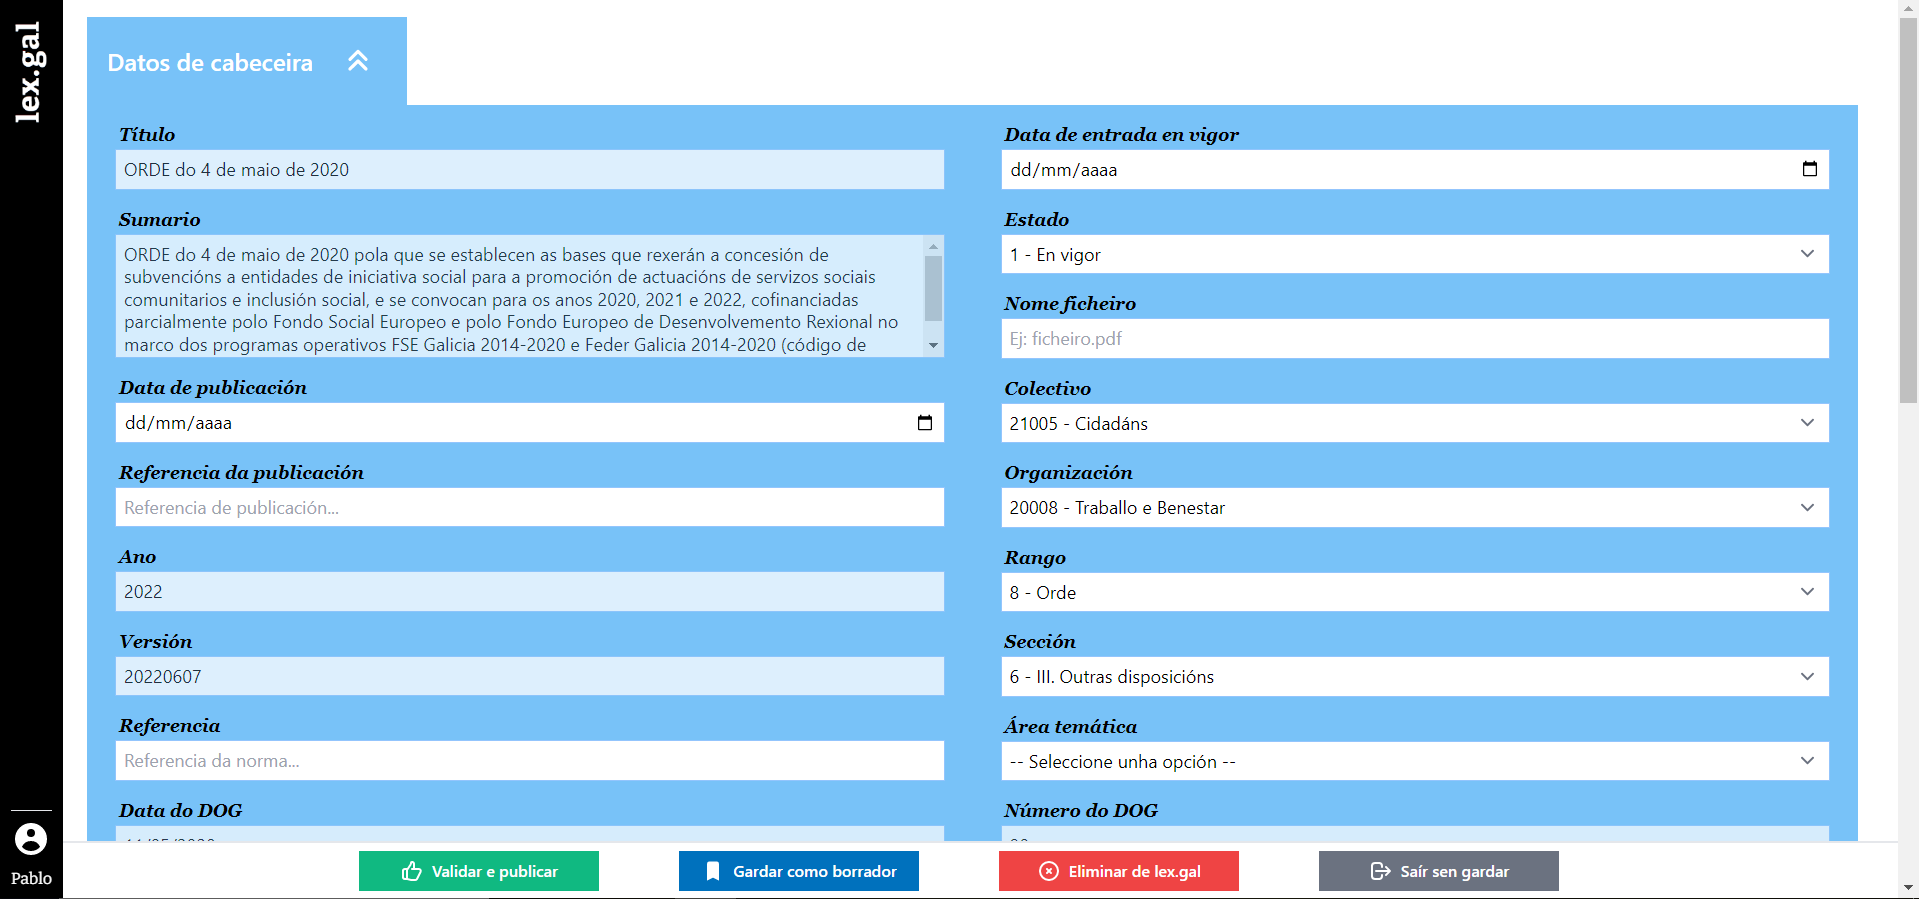
\includegraphics[width=15cm]{figuras/manualUsuario/EditarCabecera.PNG}}
\caption{Datos de cabecera de una ley de lex.gal.}
\label{enlaceCabeceraLexGal}
\end{figure}

Si se pincha en el botón de ``Previsualizar'' que se ve en la \hyperref[enlaceCabeceraLexGal]{Figura B.10}, se redirige a la página de previsualización de la ley que se está editando en lex.gal. Esta sección aparece explicada en la \hyperref[PPrevisualizacionLexGal]{Sección B.5. Página de previsualización de una ley de lex.gal}.

Si se realiza click derecho sobre cualquier párrafo del texto, se mostrará un menú donde podremos copiar o pegar contenido, proponer un cambio o añadir una anotación al párrafo.

\begin{figure}[H]
\centerline{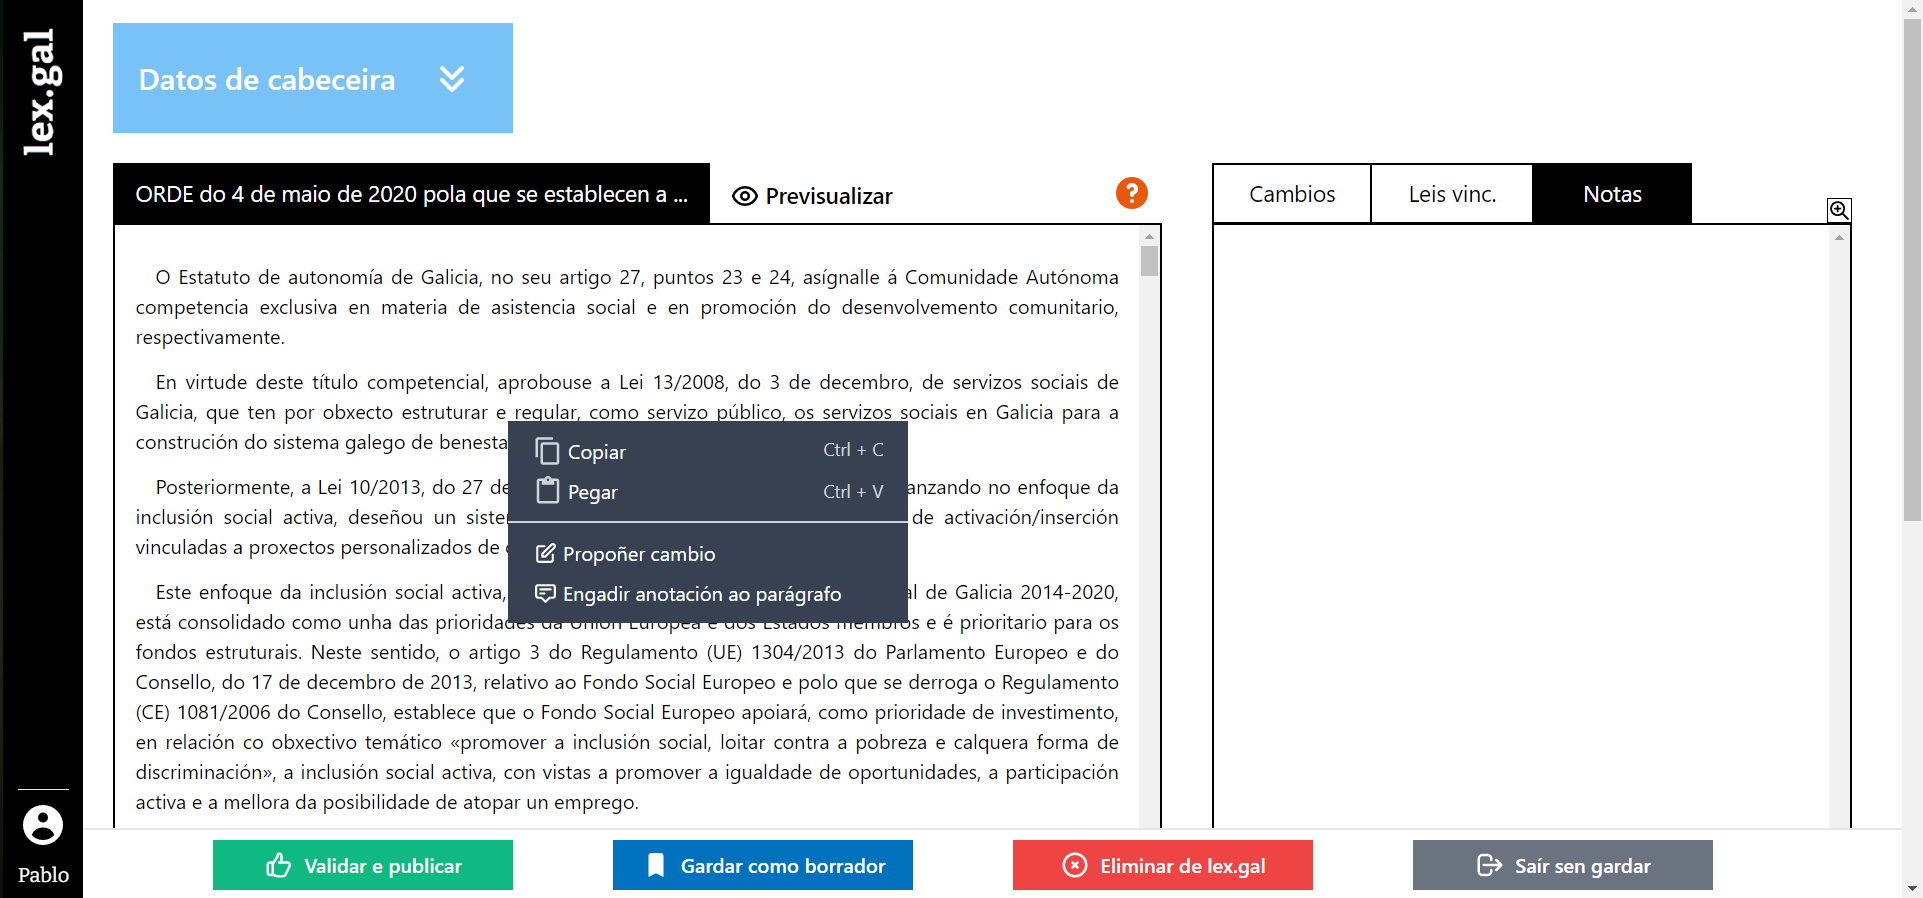
\includegraphics[width=12cm]{figuras/manualUsuario/EditarContextMenu.PNG}}
\caption{Menú de edición de un párrafo.}
\label{enlaceContextMenuLexGal}
\end{figure}

Si pinchamos en el botón ``Propoñer cambio'' de la \hyperref[enlaceContextMenuLexGal]{Figura B.11}, se abrirá una pestaña como la siguiente, donde podremos proponer un cambio. El cambio se almacenará en la pestaña de cambios de la derecha de la página, el cual puede ser desplegado para ver el cambio. Se podrá ver en el texto principal con un fondo de color verde.

\begin{figure}[H]
\centerline{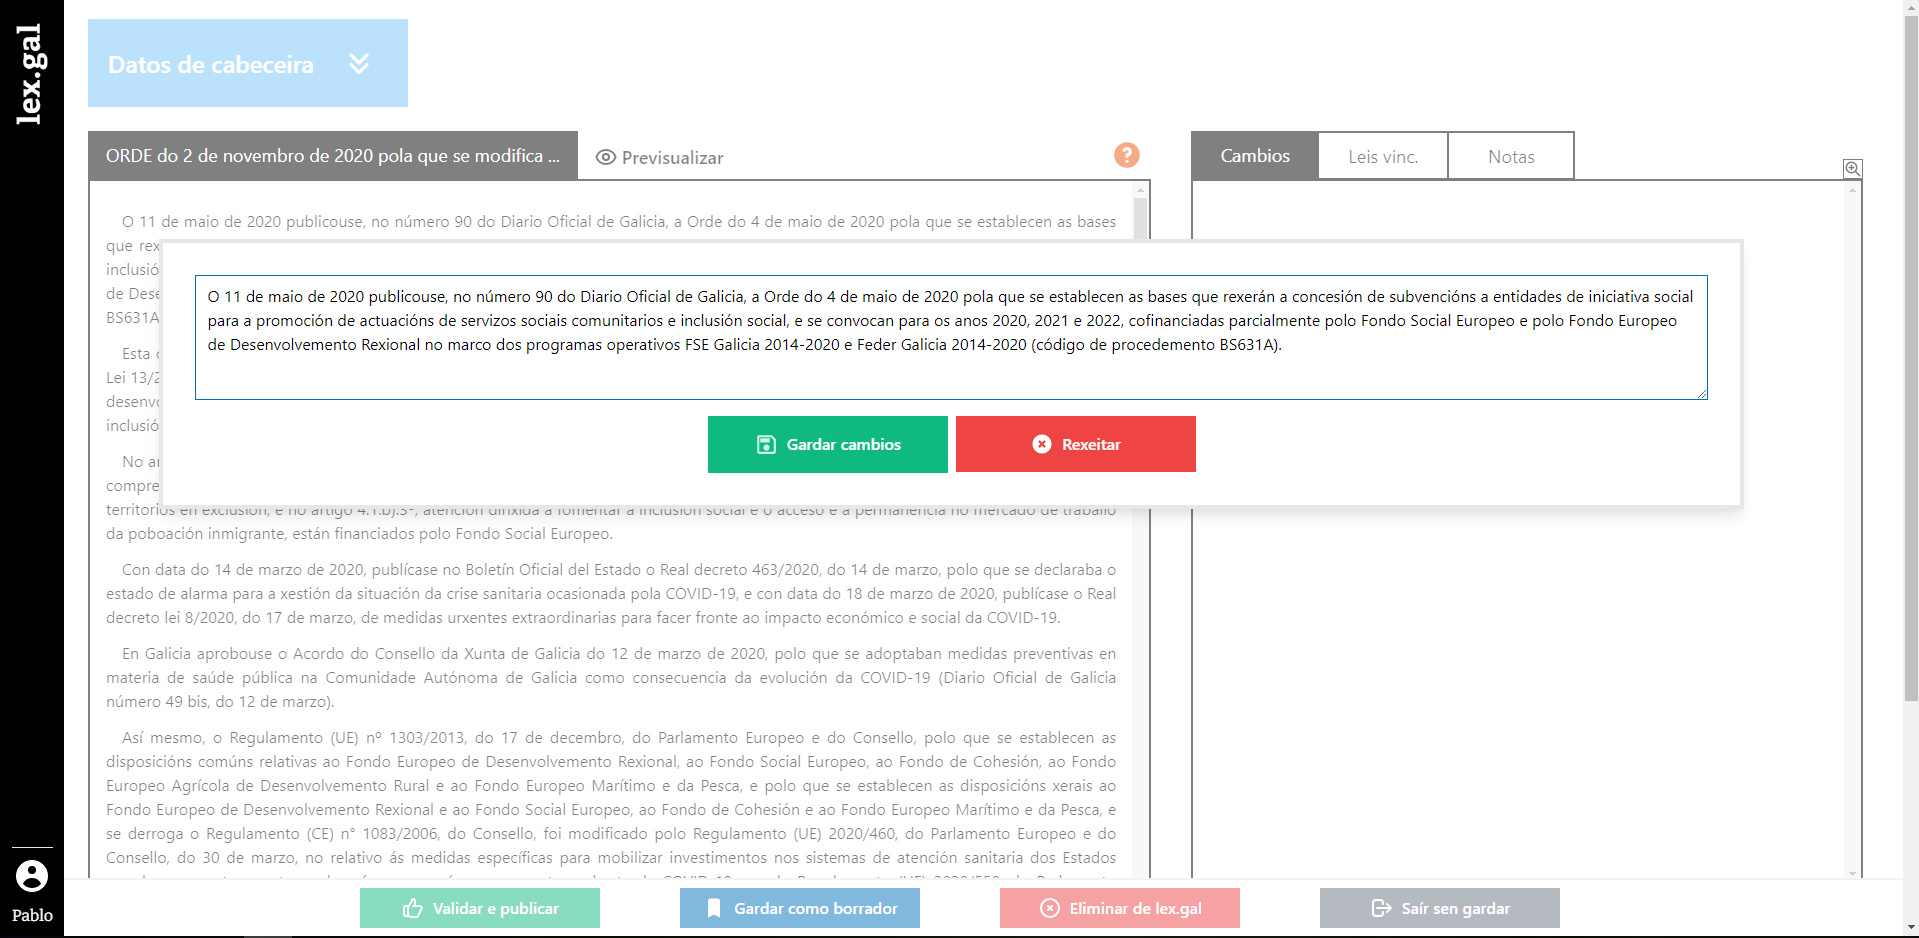
\includegraphics[width=12cm]{figuras/manualUsuario/Cambios.PNG}}
\caption{Pestaña de edición de un párrafo.}
\label{enlaceCambios}
\end{figure}

\begin{figure}[H]
\centerline{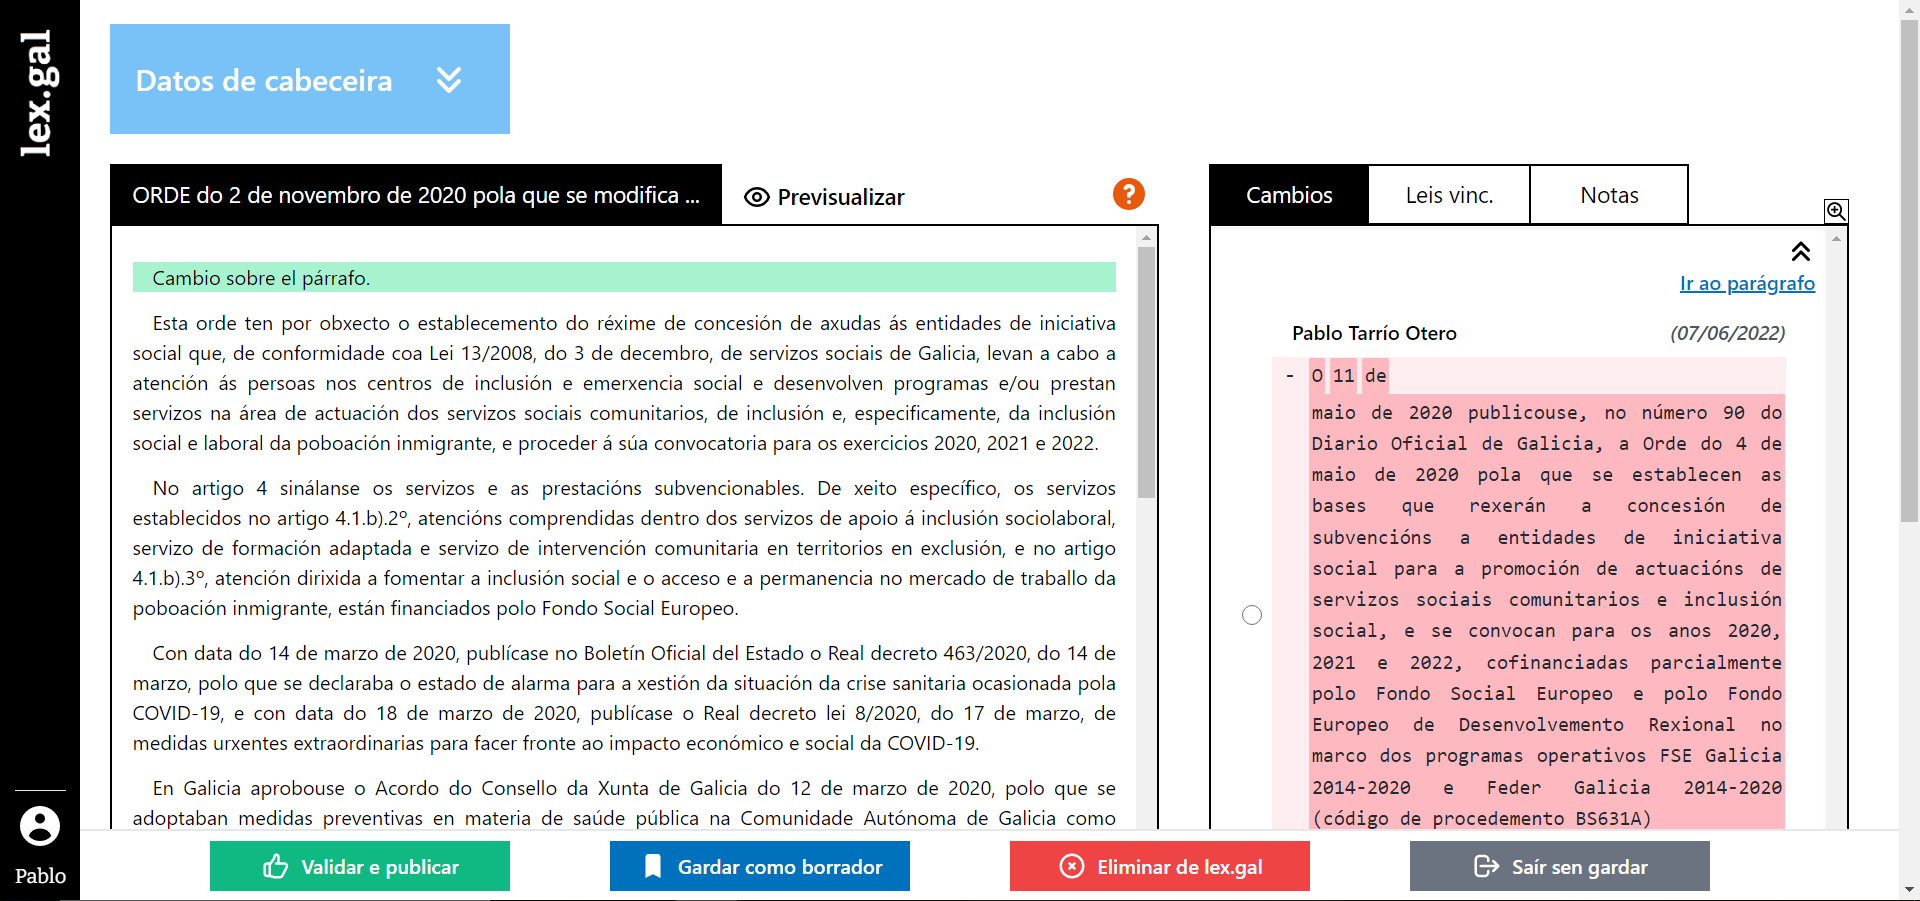
\includegraphics[width=15cm]{figuras/manualUsuario/PestanaCambios.PNG}}
\caption{Pestaña con un cambio introducido.}
\label{enlacePestanaCambios}
\end{figure}

Se muestra en las figuras \hyperref[enlaceCambios]{Figura B.12} y \hyperref[enlacePestanaCambios]{Figura B.13} el resultado de realizar un cambio.
\\

Si pinchamos en el botón ``Engadir anotación ao parágrafo'' de la \hyperref[enlaceContextMenuLexGal]{Figura B.11}, se abrirá una pestaña como la siguiente, donde podremos añadir una anotación al párrafo. La anotación se almacenará en la pestaña de notas de la derecha de la página, el cual puede ser desplegado para ver la nota completa y añadir comentarios sobre ella. Se podrá ver en el texto principal con un fondo de color naranja.

\begin{figure}[H]
\centerline{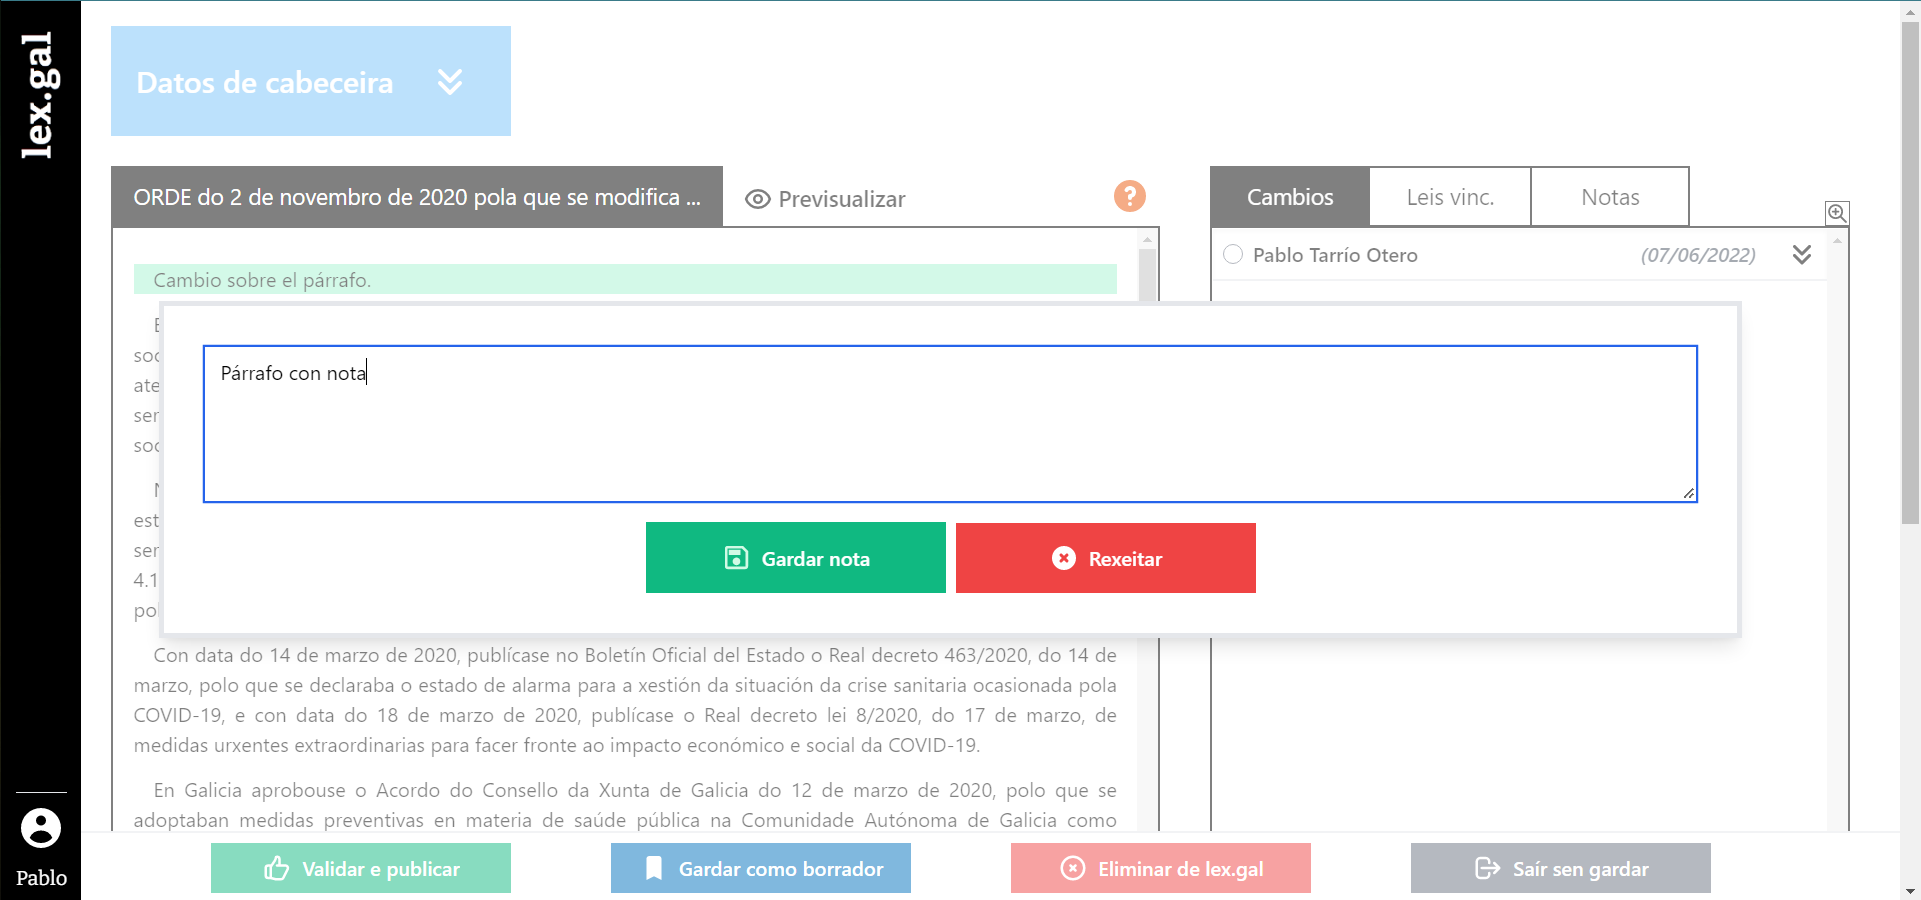
\includegraphics[width=15cm]{figuras/manualUsuario/Notas.PNG}}
\caption{Pestaña para añadir una nota a un párrafo.}
\label{enlaceNotas}
\end{figure}

\begin{figure}[H]
\centerline{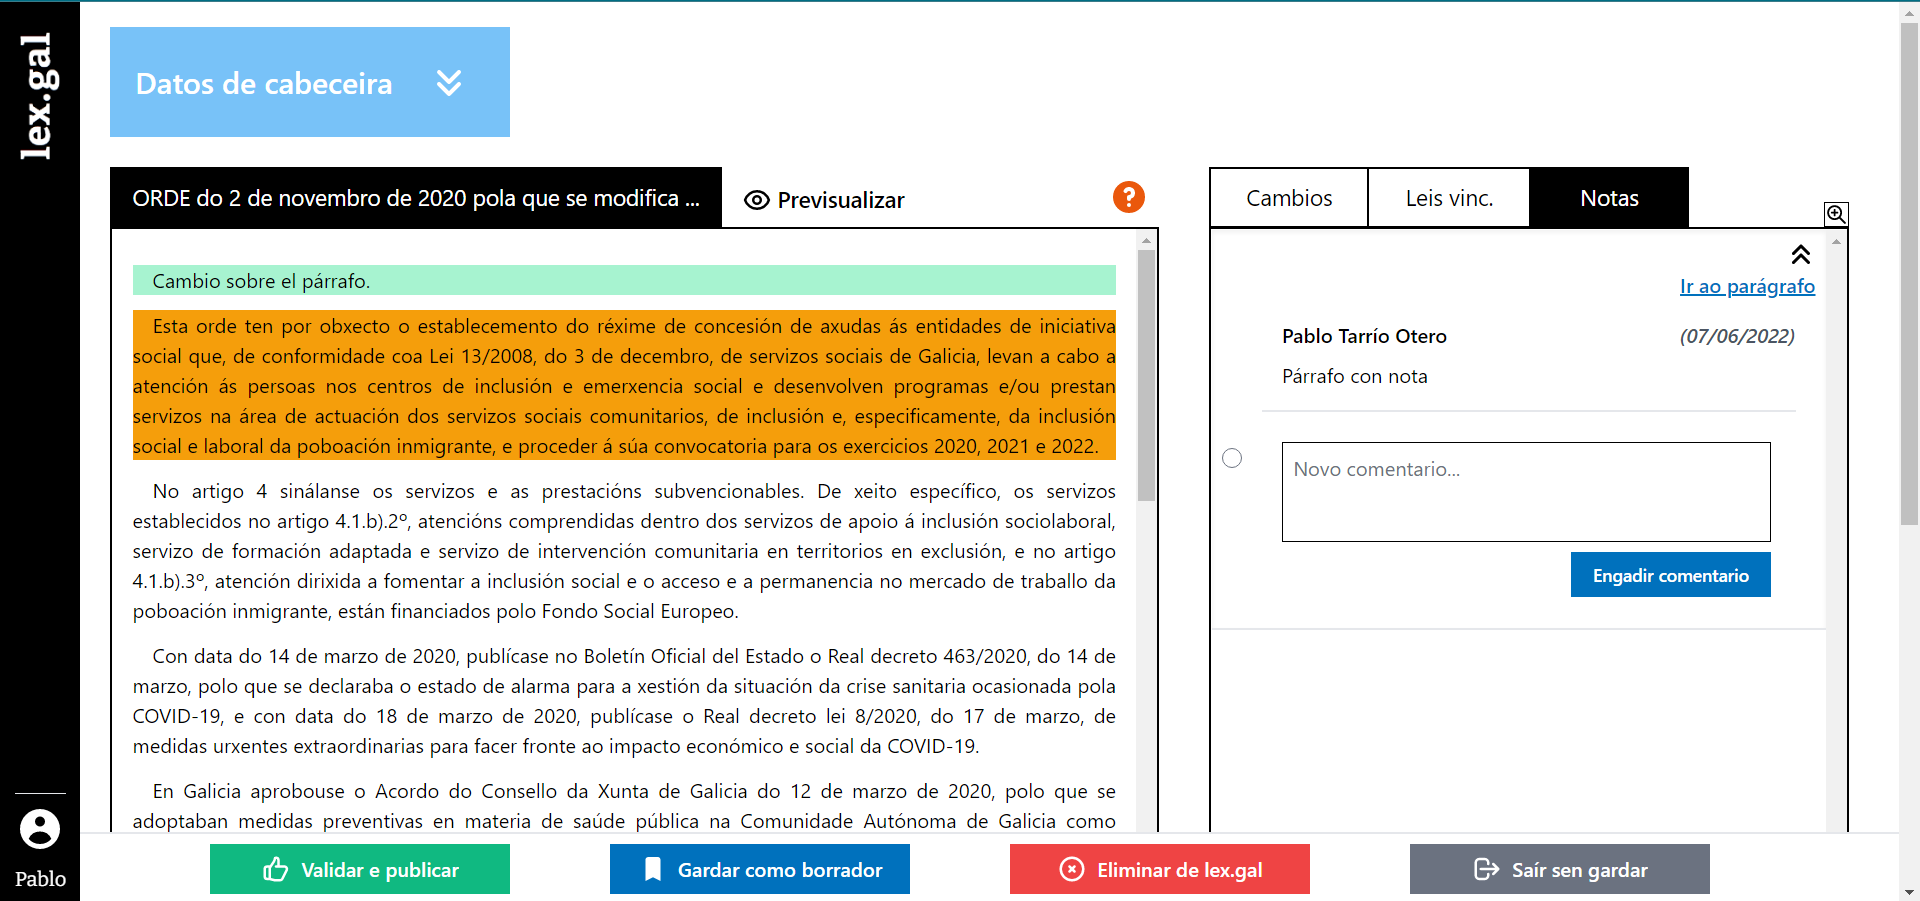
\includegraphics[width=13cm]{figuras/manualUsuario/PestanaNotas.PNG}}
\caption{Pestaña con una nota introducida.}
\label{enlacePestanaNotas}
\end{figure}

Se muestra en las figuras \hyperref[enlaceNotas]{Figura B.14} y \hyperref[enlacePestanaNotas]{Figura B.15} el resultado de añadir una anotación.
\\

En ambos casos (cambios y notas), se podrá ir al párrafo donde se ha añadido, resolver/descartar una selección de cambios/notas y resolver/descartar todos los cambios/notas.
\\

En caso de presionar sobre la pestaña de ``Leis vinc.'', se podrán observar las leyes vinculadas a una ley. En caso de poder modificar una ley vinculada, se podrá pinchar sobre esta, accediendo a la pestaña de leyes vinculadas, explicada en la \hyperref[PPrevisualizacionLexGal]{Sección B.7. Pestaña de edición de leyes vinculadas}. En caso de querer añadir una nueva ley vinculada, se abrirá una pequeña sección donde añadir la ley.

\begin{figure}[H]
\centerline{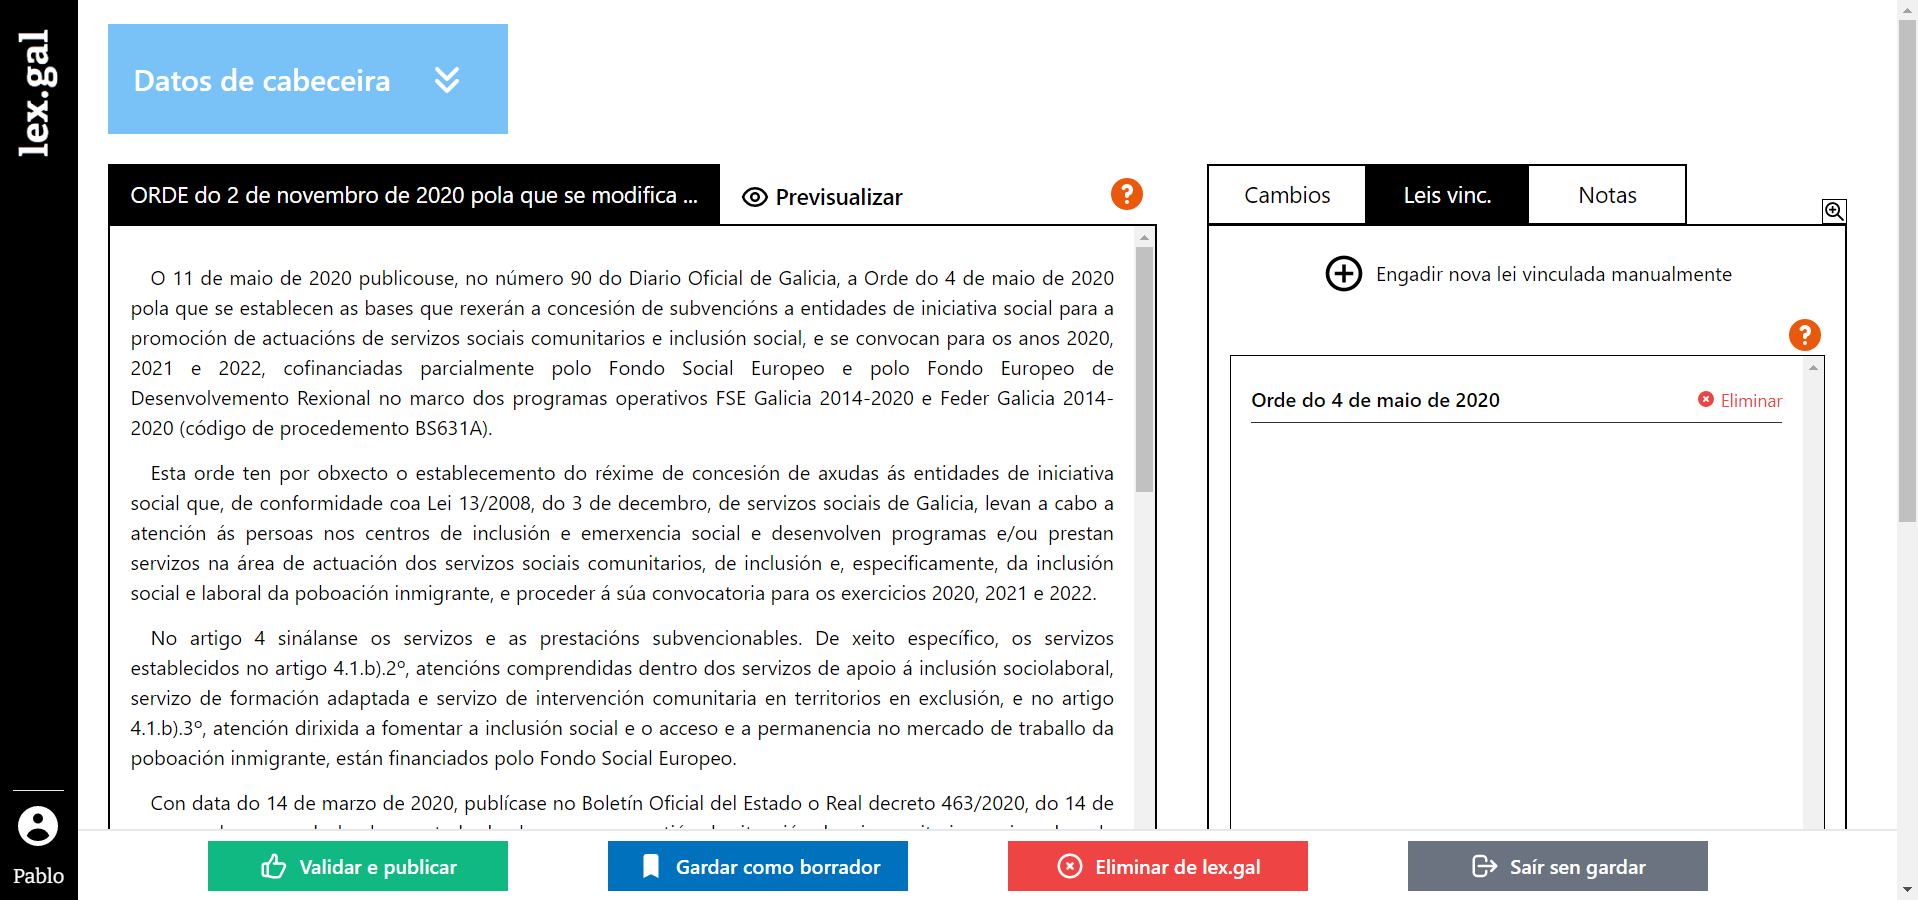
\includegraphics[width=13cm]{figuras/manualUsuario/LeyesVinculadas.PNG}}
\caption{Apartado de leyes vinculadas.}
\label{enlaceLeyesVinculadas}
\end{figure}

Para finalizar con esta página, se puede validar y publicar una ley, o también guardar como borrador (realizan la misma operación pero guardan con distintos estados la ley principal y sus leyes vinculadas), se puede eliminar una ley o se puede salir sin guardar, siendo redirigido siempre a la página principal. Y además, se muestra un mensaje de aviso antes de realizar cada operación. Todo ello se muestra en la \hyperref[enlaceLeyesVinculadas]{Figura B.16}.
\\

\begin{figure}[H]
\centerline{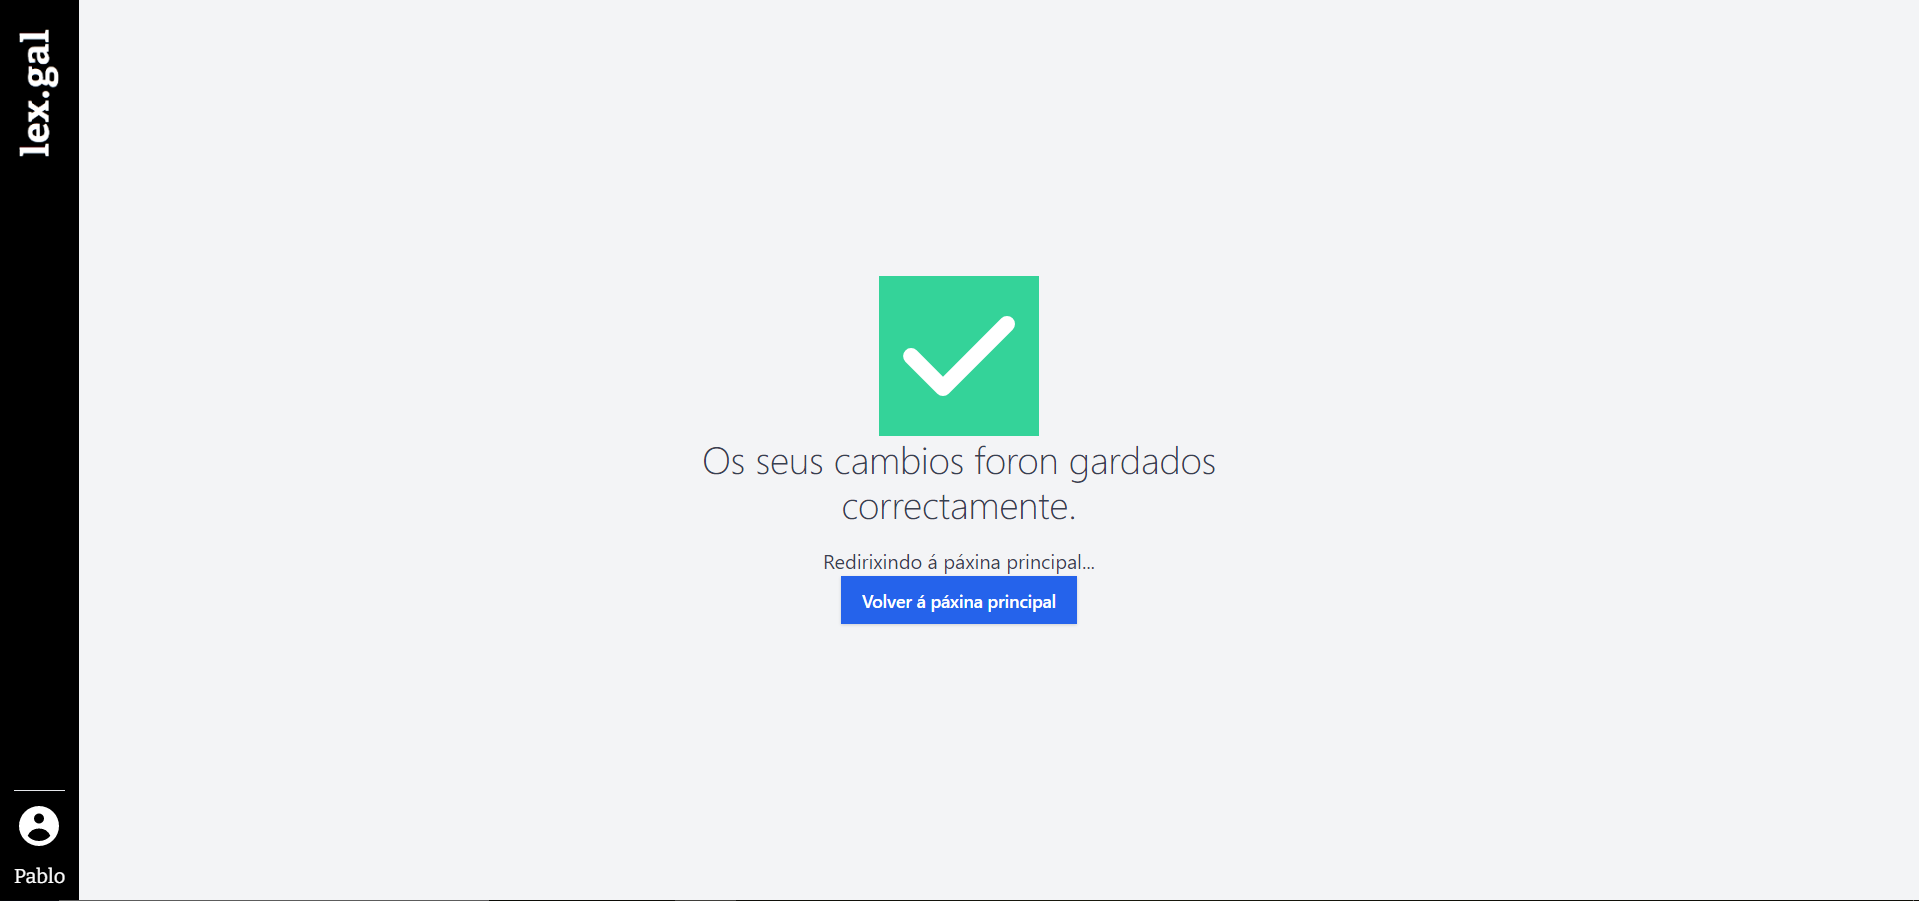
\includegraphics[width=15cm]{figuras/manualUsuario/MensajeGuardado.PNG}}
\caption{Mensaje de cambios guardados.}
\label{enlaceCambiosGuardados}
\end{figure}

En el caso de ``Validar e publicar'' o ``Gardar como borrador'', se mostrará el siguiente mensaje como indica la \hyperref[enlaceNotas]{Figura B.17}:

\begin{figure}[H]
\centerline{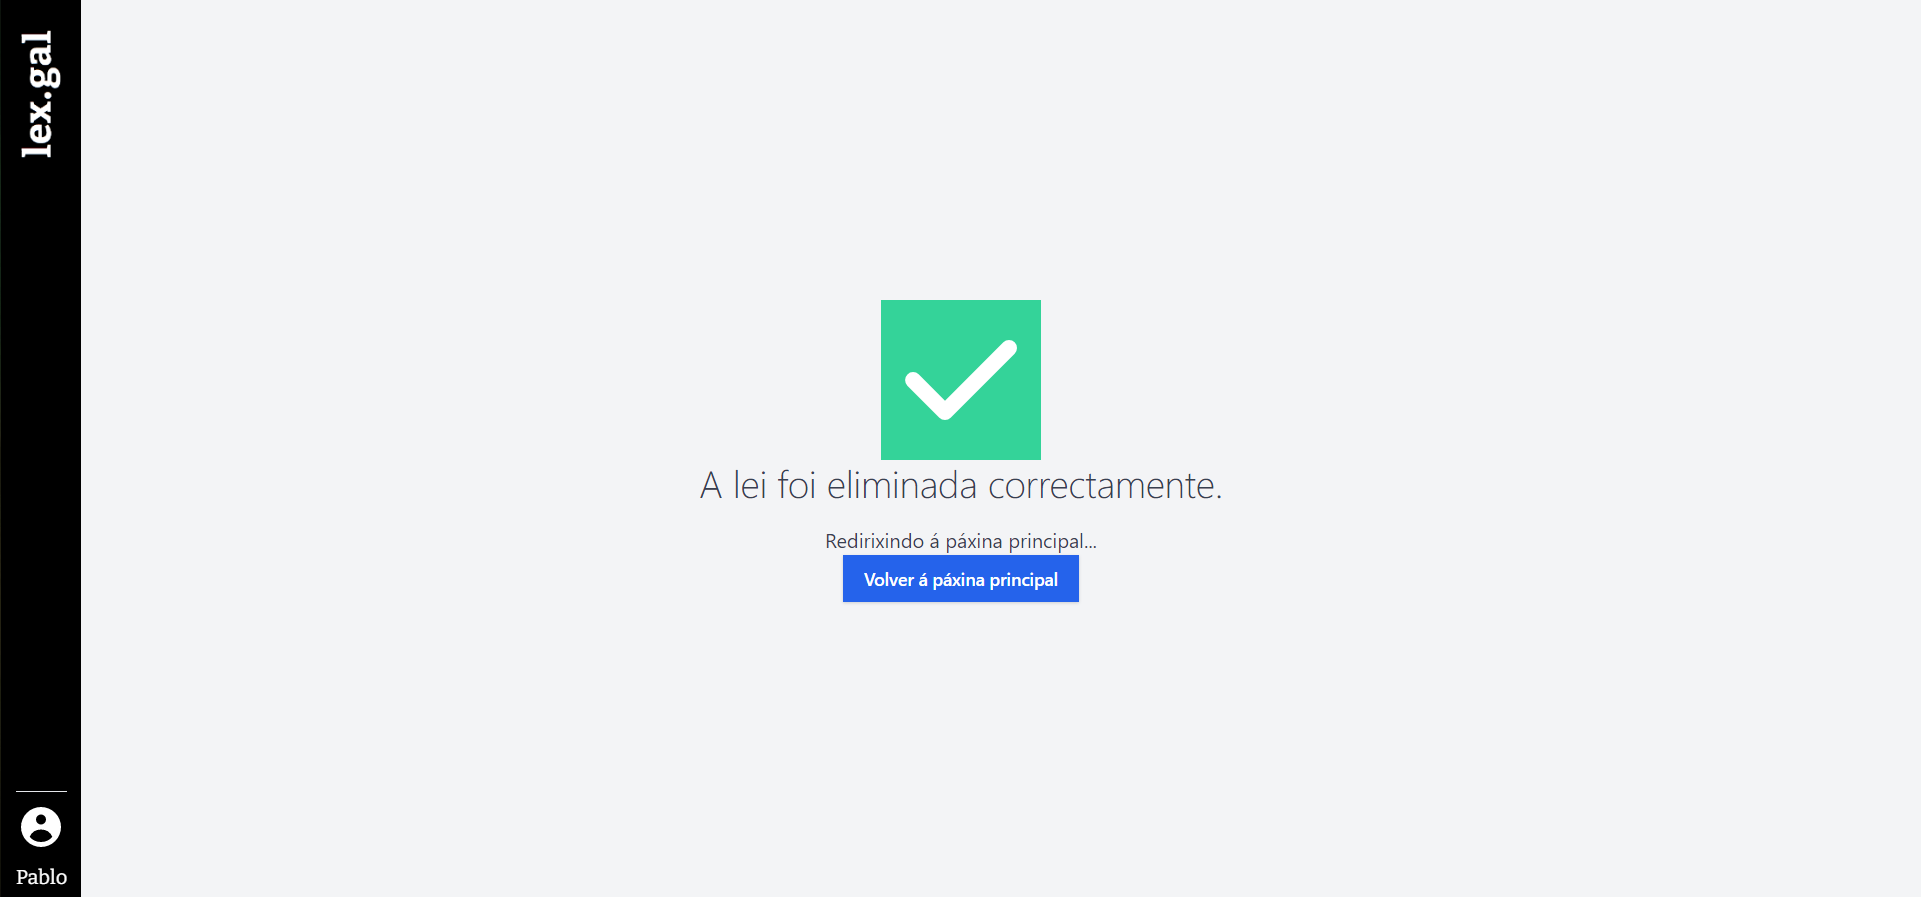
\includegraphics[width=15cm]{figuras/manualUsuario/MensajeEliminada.PNG}}
\caption{Mensaje de ley eliminada.}
\label{enlaceLeyEliminada}
\end{figure}

En el caso de ``Eliminar de lex.gal'', se mostrará el siguiente mensaje como indica la \hyperref[enlaceNotas]{Figura B.18}: